\chapter{Az ókori Egyiptom művészete} % Introduction
\label{ch:1_okri_egyiptom}

\section{Az ókori egyiptom társadalmi felépítése, hiedelemvilága, művészeti korszakai és emlékei}

\vspace{0.5cm}

\tcbox[left=0mm,right=0mm,top=0mm,bottom=0mm,boxsep=0mm,
toptitle=0.5mm,bottomtitle=0.5mm,title=\centering{A tétel adatai}]{%
	
	\begin{tabular}{| p{0.25\textwidth} | p{0.75\textwidth} |}
		
		\centering{\textbf{Tétel teljes címe}}
		&
		Mutassa be az ókori Egyiptom társadalmi felépítését, hiedelemvilágát! Ismertese az ókori egyiptomi művészet korszakait, az építészet, szobrászat és festészet ránk maradt emlékeinek jellegzetességeit!
		\\\hline
		
		\centering{\textbf{Jegyzetek}}
		&
		\begin{compactitem}
			\item Az ókori egyiptomi művészet korszakai, földrajzi, társadalmi környezete.
			\item A sír- és templomépítészet típusai, felépítése, jellmzői.
			\item A szobrászat, a festészet és tárgykultúra jellemzői és stílusjegyei.
		\end{compactitem}
\end{tabular}}\hfill

\subsection*{Földrajzi elhelyezkedés}

\begin{figure}[H]
	\centering
	\tcbox[colback=gray!85!black,
	left=0mm,right=0mm,top=0mm,bottom=0mm,boxsep=1mm,toptitle=0.5mm,bottomtitle=0.5mm,
	title=\centering{Az ókori Egyiptom a Nílus mentén feküdt}]{
		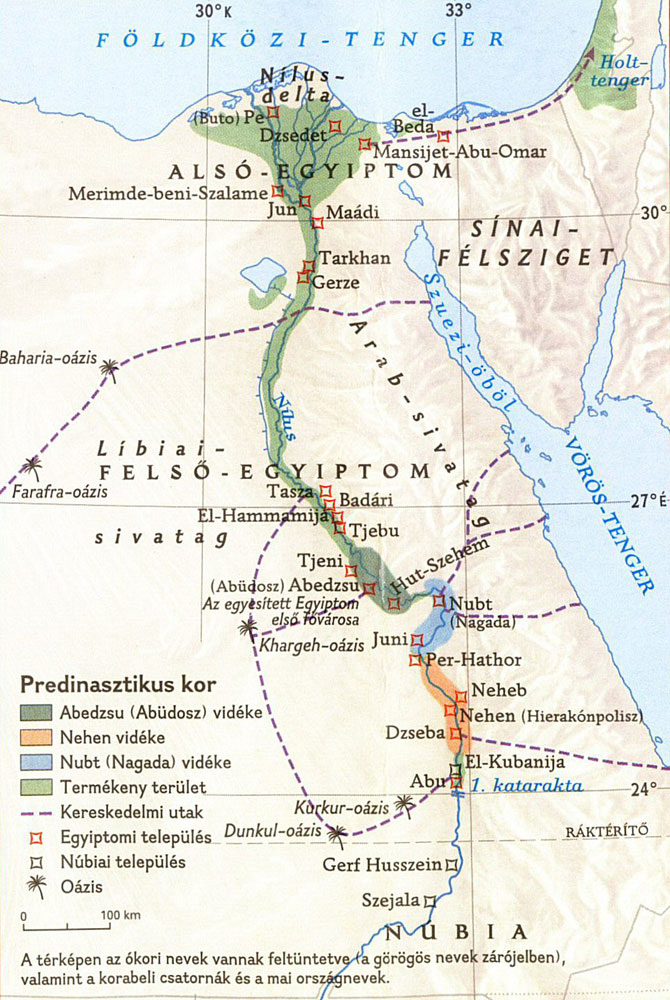
\includegraphics[width=0.9\linewidth]{images/01/egyiptom_terkep}}
	\captionsetup{labelformat=empty}
	\caption{}
\end{figure}

Egyiptom éghaljata alapvetően sivatagos, ezért a kultúra a \textbf{Nílus mentén}, annak partján 5-10 km-es szélességben, több mint 1 000 km hosszan alakult ki.

Ezen ókori civilizáció kialakulásának feltétele a folyó éltető ereje volt: a Nílus. A folyó vetés előtt, júliustól novemberig áradt, termékeny iszapot terítve szét, tápanyagban gazdaggá téve a talajt és lehetővé tette az \textbf{elárasztásos gazdálkodás}t.

A terület földrajzilag és kezdetben politikailag is két részre tagolódott. \textbf{Alsó Egyiptom} északon, a Nílus deltatorkolatánál feküdt a sík vidéken. \textbf{Felső Egyiptom} attól délebbre, a magasabban fekvő területeken, a Nílus mentén hosszan kanyargó partszakaszon helyezkedett el.

\subsection*{Társadalmi felépítés}

\begin{tcolorbox}[enhanced,colframe=gray!50!white,
	colbacktitle=gray!15!white,
	coltitle=gray!50!black,
	borderline={0.5mm}{0mm}{gray!15!white},
	borderline={0.5mm}{0mm}{gray!50!white,dashed},
	attach boxed title to top center={yshift=-2mm},
	boxed title style={boxrule=0.4pt},
	title=Az ókori Egyiptom társadalmi felépítése]{
			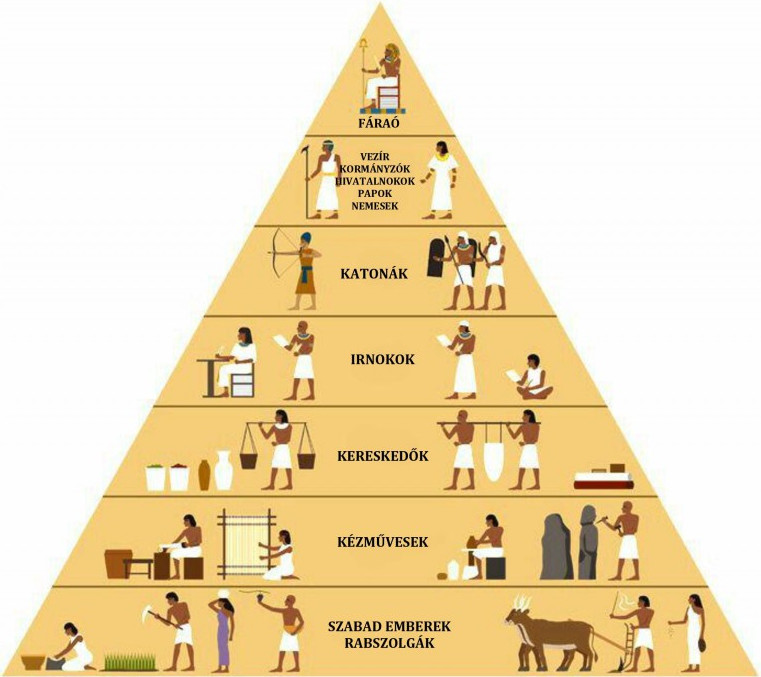
\includegraphics[width=0.9\linewidth]{images/01/egyiptomi_tarsadalom}}
\end{tcolorbox}

Az állam élén a korlátlan hatalommal rendelkező \textbf{fáraó} állt. Az előkelőket a származás szerinti arisztokrácia alkotta, belőlük kerültek ki a főtisztviselők. Az államigazgatás és az igazságszolgáltatás vezetője a vezér. A gazdasági élet irányítószerve a kincstár, az államgépezet működését az írnokok biztosították.

A közigazgatási egységek a nomoszok (kerületek), élükön a nomarkhoszokkal (kormányzókkal). A közrendűeket két réteg alkotta: a parasztok - a föld használata fejében terménnyel és közmunkával adóztak -, és a kézművesek. A házi rabszolgák a hadifoglyokból kerültek ki.\\

\begin{compactitem}
	
	\item\textbf{ Fáraó}: a trón betöltése általában a primogenitura elve (elsőszülött öröklése) történik.\\
	\textit{A fáraó volt a hadsereg főparancsnoka, az államigazgatás és a kincstár feje, valamenynyi templom főpapja és a legfőbb bíró. Mindezeken túl úgy gondolták, hogy rajta múlik az ország termékenysége. Ő tette a földeken az első kapavágást, és ő kezdte meg az aratást.}
	
	\item\textbf{ Papi arisztokrácia}\\
	\textit{A papok - egyiptomi felfogás szerint - csupán az uralkodót helyettesítették kultikus funkcióiban. Hisz a legfőbb pap a fáraó volt! Az egyiptomi papság két fontos funkciót látott el: az istenek kultuszának szolgálatát a templomokban és a halottakról való gondoskodást, az áldozatok bemutatását.}
	
	\item \textbf{Katonai arisztokrácia}\\
	\textit{A fáraó hatalmának alapja a felügyelete alatt álló oikosz-gazdaság és a zsoldos hadsereg volt mely akatonai arisztokrácia megszilárdulásával vált lehetővé. A katonai tisztségviselők elsősorban a társadalom tehetősebb képviselői voltak: előkelők, nagyobb földbirtokosok.}
	
	\item \textbf{ Írnokok} (tisztviselők) (nyilvántartás, adóztatás)\\
	\textit{Az egyiptomi állam legfontosabb hivatalnoka volt. Az irnokok készítették a legfontosabb feljegyzéseket, összeírásokat, a különböző vallási, orvosi, irodalmi szövegeket. Az írástudás minden hivatal elnyerésének feltétele volt. Egy-egy előkelő tucatnyi irnokot foglalkoztatott, s az írnokból akár magas méltóság is válhatott.}
	
	\item \textbf{Kézművesek}\\
	\textit{A Der-el-Medinában élő, kézműves férfiaknak és nőknek tíz napos időszakokra el kellett hagyniuk a várost és családjukat, hogy dolgozni menjenek oda, ahová a fáraó és legfőbb tanácsadói parancsolták. Rövid pihenési időszak után a munkások újabb tíz napot dolgoztak.}
	
	\item\textbf{ Közrendű szabadok}\\
	\textit{A közrendű szabadok foglalkozás szerint földművesek, kézművesek és kereskedők lehettek. A "félszabadok" az ún. királyi munkások, a földbirtokhoz kötött - főleg - parasztok.
	Fontos tény továbbá, hogy a piramisokat nem rabszolgák építették, hanem a közrendű, szabad népesség.}

	\item \textbf{Parasztok}: középítkezések az áradások idején
	
	\item \textbf{Rabszolgák}\\
	\textit{A rabszolgák döntően hadjáratok folyamán kerültek Egyiptomba. Már az i.e. 2700 kö-rül keletkezett „ palermói kő „ is beszámolt arról, hogy egy núbiai hadjárat  után 7000 foglyot hurcoltak az országba.}
\end{compactitem}

\vspace{0.5cm}

Az ókori egyiptomiak úgy hitték, hogy hajdanában nem voltak földi királyok, hanem maguk az istenek uralkodtak az ország felett. Ozirisz volt az, aki földművelésre tanította az embereket. Az ő felesége volt Ízisz, fiuk pedig Hórusz, a sólyomisten. A hór szó valójában magasröptűt, magasságot is jelentett, ezért származtatták magukat tőle az uralkodók. \textbf{Az egyiptomiak királyaikat tehát az istenek földi képviselőjének tekintették.}

\subsection*{Írásmód}

	\begin{wrapfigure}{r}{0.3\textwidth}
		\tcbox[colback=darkgray!85!black,
		left=0mm,right=0mm,top=0mm,bottom=0mm,boxsep=1mm,toptitle=0.5mm,bottomtitle=0.5mm,
		title=\centering{A rosettei kő}]{
		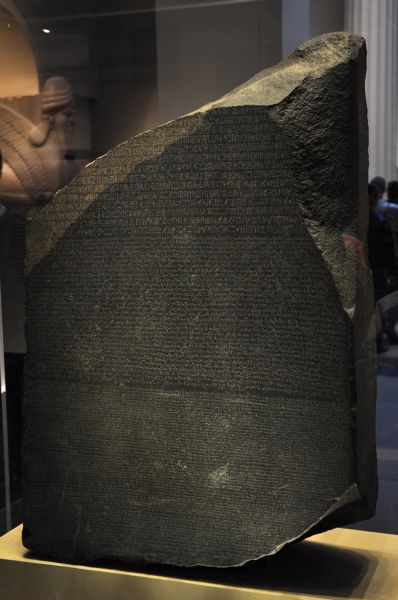
\includegraphics[width=1.0\linewidth]{01/rosetti_ko}
	}
	\end{wrapfigure}

	A legismertebb írásmód a \textbf{hieroglifa} (a szó görög eredetű és „szent vésetet” jelent), \textbf{elsősorban a falakra került és a kultuszhoz} [= a vallásgyakorlat, a vallásos szertartások összessége] \textbf{kapcsolódott}.
	
	Maguk az egyiptomiak írásukat a \textit{medu netjeru}, „az istenek szavai” névvel illették, ezzel is utalva a legendára, mely feltalálását Thot istennek tulajdonítja.
	
	A hieroglifa-írást 1822-ben fejtette meg Francois Champollion [sampolion] francia tudós, az ún. rosette-i kő alapján, amely egy olyan kőtábla volt, amin ugyanaz a szöveg három nyelven volt olvasható többek közt görög betűkkel.

	\begin{figure}[H]
		\centering
		\tcbox[colback=white!85!black,
		left=0mm,right=0mm,top=0mm,bottom=0mm,boxsep=1mm,toptitle=0.5mm,bottomtitle=0.5mm,
		title=\centering{A hieroglif írás}]{
			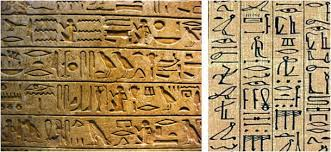
\includegraphics[width=0.9\linewidth]{images/01/hieroglifa}}
		\captionsetup{labelformat=empty}
		\caption{}
	\end{figure}

	Az írás leggyakoribb alapanyaga - a sírfalakon kívül - a papirusztekercs volt. A háromszög keresztmetszetű papirusznád belső rostjait kivették, hosszú csíkokra vágták, 6 napig vízbe áztatták, függőlegesen majd ezekre keresztbe egymásra helyezték a csíkokat (tulajdonképpen egy fonatot hoztak létre). Majd újabb 6 napon keresztül összepréselték, kiszárították, végül a lapokat a végüknél egymáshoz ragasztották, így jött létre az összegöngyölhető tekercsforma a könnyebb tárolhatóság érdekében.
	

\subsection*{Hiedelemvilág}

\subsection*{Művészeti korszakok}

Egyiptom történelmének nagy részét három „birodalmi” szakaszra lehet osztani: az óbirodalmi szakaszra, a középbirodalmi szakaszra és az újbirodalmi szakaszra. Ezeket rövidebb átmeneti időszakok választották el egymástól. Az „átmeneti” szó itt arra utal, hogy ezekben az időkben Egyiptom nem állt egységes politikai uralom alatt, hanem más, erősebb birodalmak uralma alá került. Az egyiptomi civilizáció alapjait jóval az Óbirodalom kora előtt a Nílus folyó partján letelepülő emberek által létrehozott öntözéses földművelés fektette le, amely a városok és specializált gazdasági tevékenységek (például a kézművesség, bányászat) kialakulásához vezetett.

Művészeti korszakokra tagolva: építeszt, szobrászat és festészet.

\cleardoublepage

\section{Az ókor meghatározó festészeti techinkái: az egyiptomi falkép}

\begin{center}
	\begin{longtable}{ | m{0.25\textwidth} | p{0.75\textwidth} | }
		
		\hline
		\multicolumn{2}{|c|}{\textbf{A tétel adatai}}
		\\ \hline
		
		\hline
		Tétel teljes címe	
		 &
		 Melyek a meghatározó festészeti technikák az ókorban? Fejtse ki, miként alakult egy egyiptomi falkép elkészítésének munkamenete, milyen alapozást, pigmenteket és kötőanyagot használtak?
		\\ \hline
		
	\end{longtable}
\end{center}